\documentclass[11pt, a4paper]{report}
%\usepackage[german]{babel}
\usepackage{listings}

%Math Library
\usepackage{amsmath}

%Images Library
\usepackage{graphicx}
\graphicspath{ {./images/} }

%General Layout
\usepackage{geometry}
\geometry{
    a4paper,
    left=20mm,
    right=20mm,
    top=20mm,
    bottom=20mm
}


%Background image
\usepackage[pages=some]{background}

%Liks of TOC
\usepackage{color}   %May be necessary if you want to color links
\usepackage{hyperref}
\usepackage{lstmisc}
\hypersetup{
    colorlinks=false, %set true if you want colored links
    linktoc=all,     %set to all if you want both sections and subsections linked
    linkcolor=blue,  %choose some color if you want links to stand out
}


\backgroundsetup{
scale=1,
color=black,
opacity=1,
angle=0,
contents={%
\hspace*{13.5cm}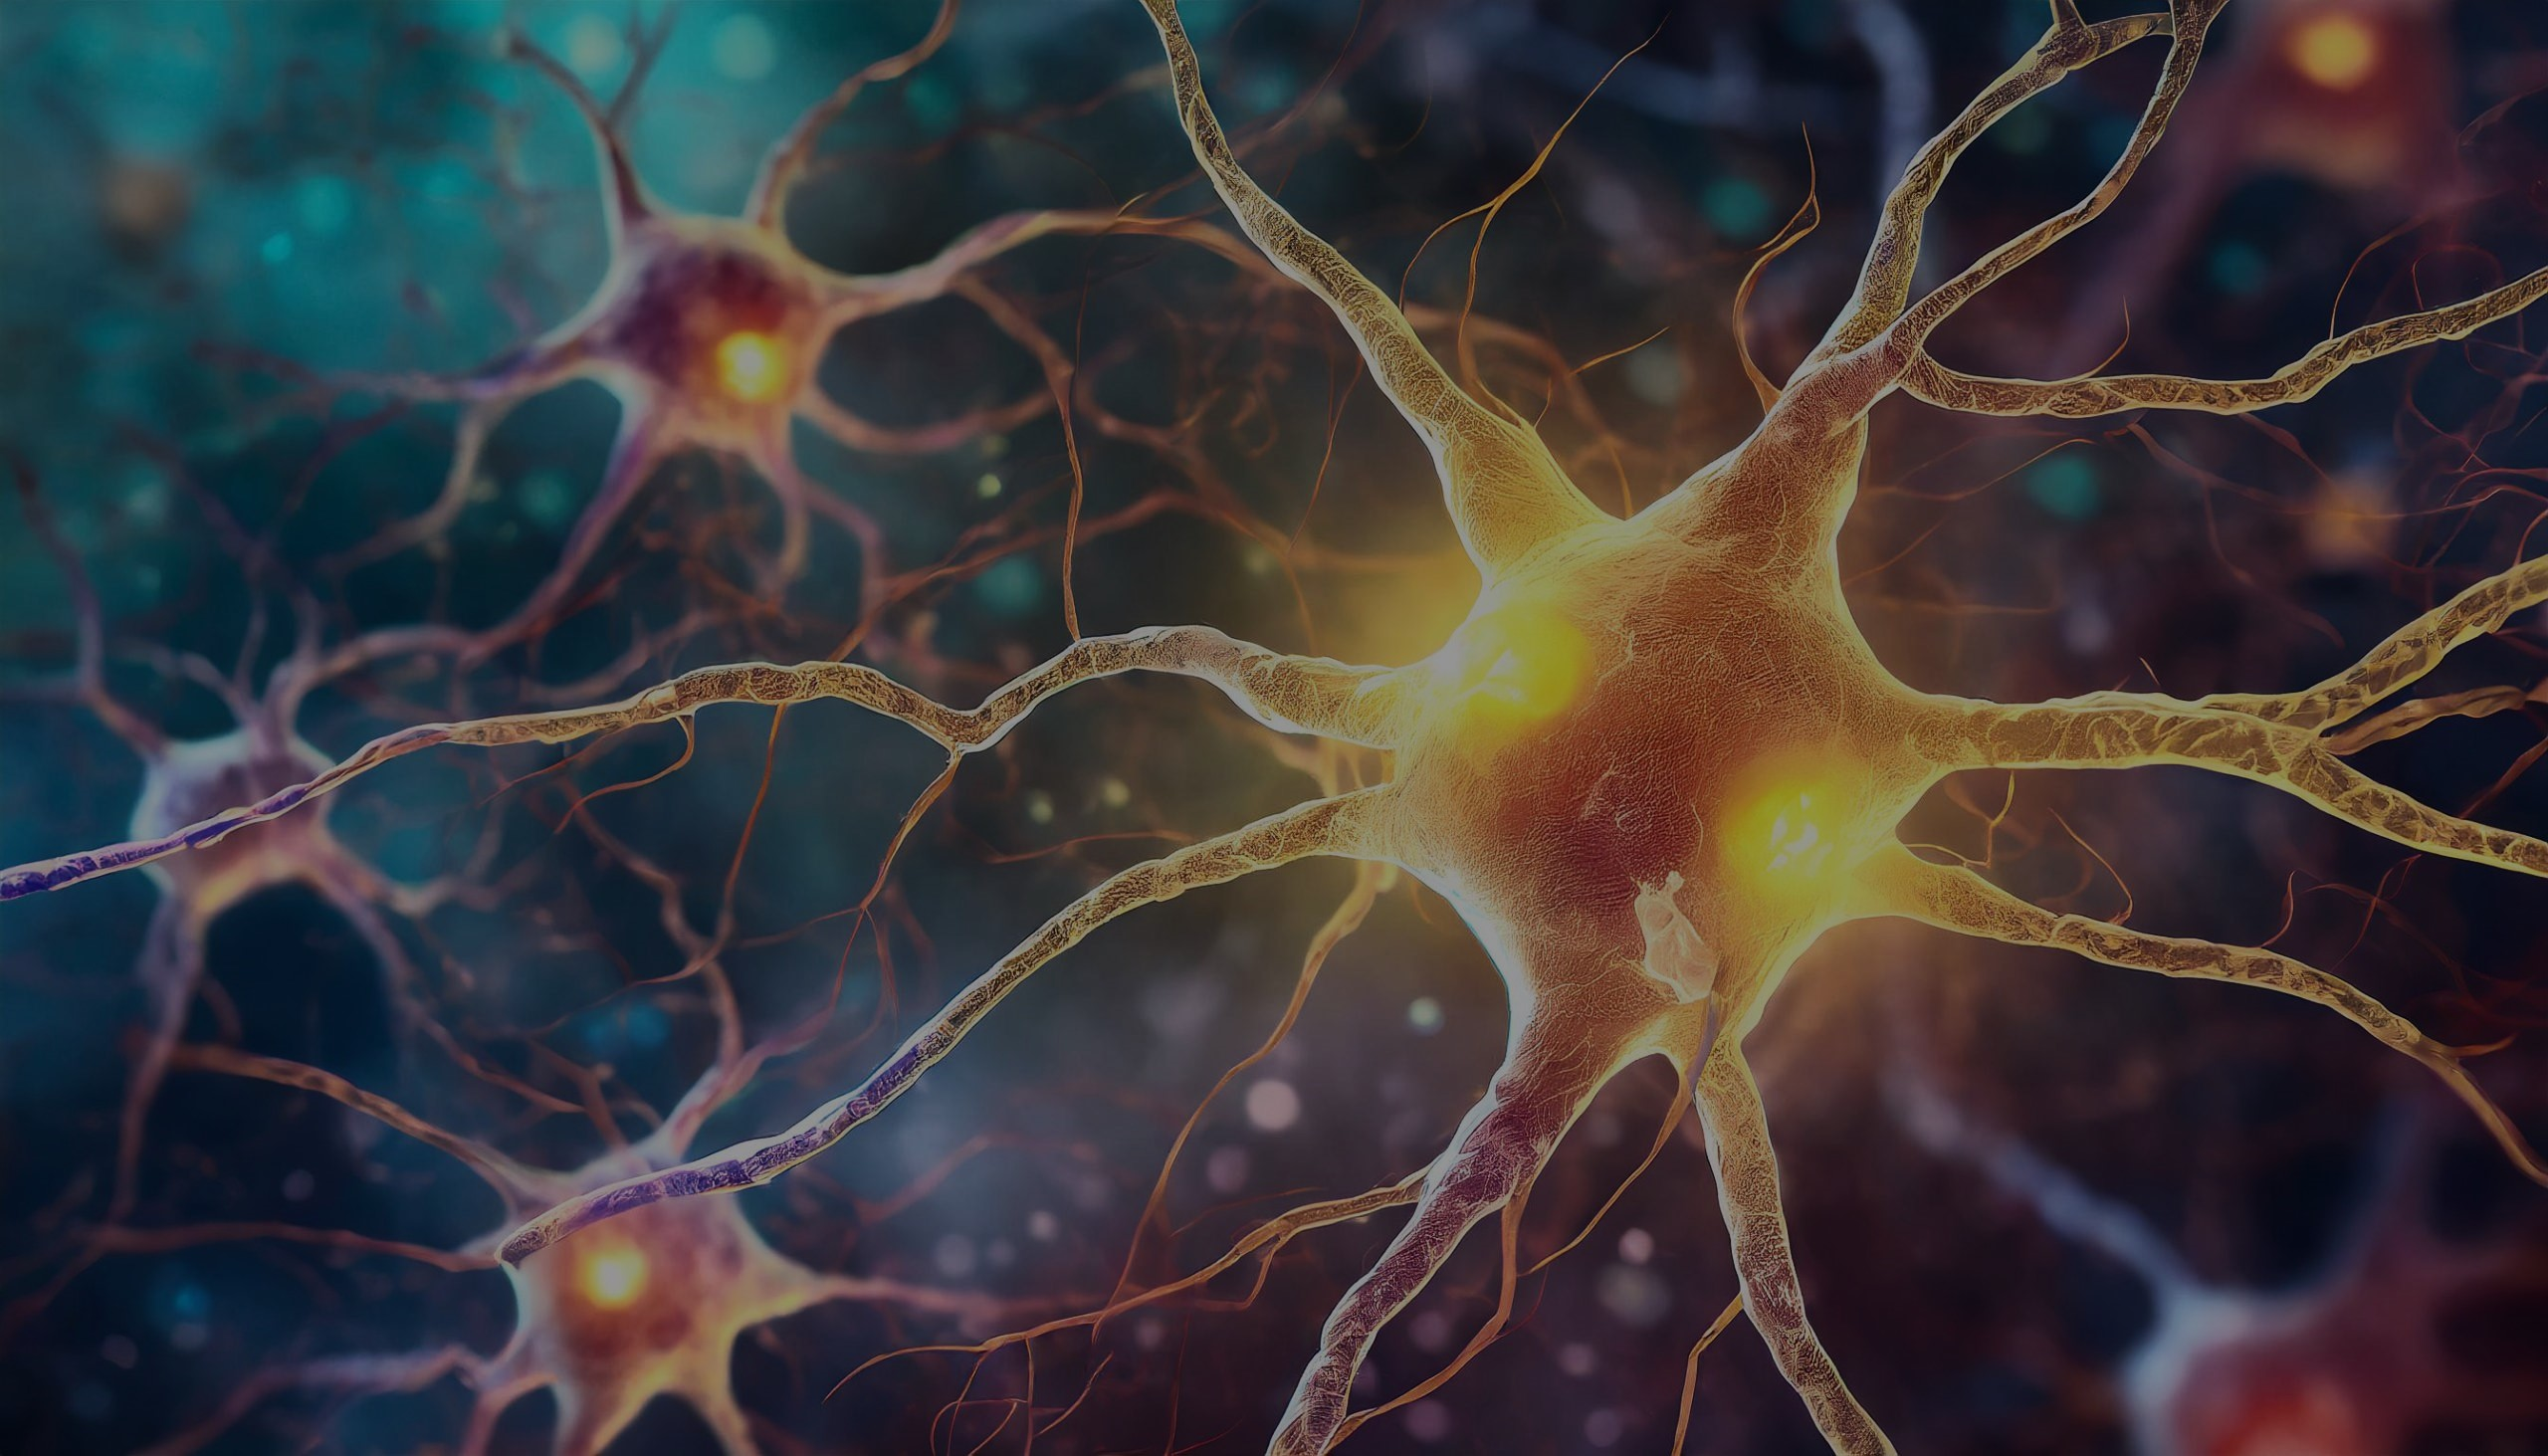
\includegraphics[width=3\paperwidth,height=\paperheight]{abstract_neurons3}
  }%
}


\begin{document}
    \pagenumbering{gobble}
    \begin{titelpage}
        \BgThispage
            \color{white} {
                \begin{center}
                    \Large \textsc{Matura Thesis}\\Kantonsschule Hohe Promenade\\
                    \rule[0.1cm]{15.8cm}{0.1mm}\\
                    \vspace{3cm}
                    \Huge \textbf{ \textsc{How can you develop \\Evolutionary Neural Networks which \\learn to play Board Games?}}\\
                    \vspace{0.8cm}
                    \Large \textit {Implementation \& Study \\of Evolutionary Neural Networks \\using the NEAT Algorithm}\\
                \end{center}
                \vspace{3cm}
                \rule[0.1cm]{15.8cm}{0.1mm}\\
                \vspace{7cm}\\
                \begin{minipage}[t]{0.47\textwidth}
                \large\textbf {Thesis By:}\\
                \end{minipage}
                \hfill
                \begin{minipage}[t]{0.47\textwidth}\raggedleft
                \large\textbf {Lucien Kissling 6e}\\
                \end{minipage}
                \begin{minipage}[t]{0.47\textwidth}
                \large \textbf {Year:}\\
                \end{minipage}
                \hfill
                \begin{minipage}[t]{0.47\textwidth}\raggedleft
                \large \textbf {2025}\\
                \end{minipage}
                \begin{minipage}[t]{0.47\textwidth}
                \large \textbf {Supervisor:}\\
                \end{minipage}
                \hfill
                \begin{minipage}[t]{0.47\textwidth}\raggedleft
                \large \textbf {Timo Schenk}\\
                \end{minipage}
                \begin{minipage}[t]{0.47\textwidth}
                \large \textbf {Co Examiner:}\\
                \end{minipage}
                \hfill
                \begin{minipage}[t]{0.47\textwidth}\raggedleft
                \large \textbf {Dr. Arno Liegmann}\\
                \end{minipage}
                \vfill
            }
        \clearpage
    \end{titelpage}
    \pagenumbering{arabic}
    \setcounter{page}{2}
    \tableofcontents
    \chapter{Introduction}
        \section{Preface}
    Ever since I got into Computer Science a few years ago, I was fascinated by the Idea of Algorithms that solved various Problems.
    Therefore, I participated in the SOI (Swiss Olympiad in Informatics) where we were taught everything about developing and programming Algorithms and their Data Structures.
    \\ \\ In recent years although, a new field of Computer Science has gained a lot of attention, where those Algorithms are not programmed by humans, but evolved by a computer.
    This field called Machine Learning immediately got my excitement and two years ago a friend of mine and I had our first practical experience with it.
    We developed a simple Neural Network, which helped us predict the color of a lego brick in front of a color sensor based on the RGB values in various lighting conditions.
    \\ \\ A Neural Network (NN) forms the basis of most Machine Learning Models and I will therefore explain it in much detail in the following Chapters.
    In simple terms, a NN is a strongly simplified artificial model of the human brain as a NN consists of an interconnected web of Neurons through which information flows and gets computed.
    \\ \\ Although the NN we developed two years ago already learned on its self, we still had to provide data for it to learn from.
    This meant that we had to manually scan the RGB values of the lego bricks and then label them with the color they represented.
    The aim of my Matura Thesis therefore is to take the idea of self learning a step further by developing Neural Networks, which don't need this kind of data with solutions predefined by humans.

        \section{Thesis Statement}
    As mentioned in the previous Section, this Thesis will explore the field of Neural Networks (NNs) that learn without data provided by humans, which is called unsupervised learning.
    The solution this Thesis will focus on is the Neuroevolution of Augmenting Topologies (NEAT) Algorithm, a combination of Neural Networks and Genetic Algorithms.
    This Algorithm was invented by Kenneth O. Stanley and Risto Miikkulainen in 2002 and has since then been used in various applications.
    In this Thesis, I develop my own simplified implementation of the NEAT Algorithm and then train it on Board Games to see how well it can learn to play them.
    The first game I will train it on is Nim, a simple game where two players take turns removing matches from different stacks.
    \\ \\ In specific, this Thesis aims to answer following questions:
    \begin{itemize}
        \item How can you develop Neural Networks that learn to play Board Games using NEAT?
        \item How do different parameters and features of the NEAT Algorithm affect the learning process?
        \item How does this Implementation of NEAT compare to other Machine Learning Algorithms?
    \end{itemize}
    \chapter{Background}
        \section{Neural Networks (NNs)}
        \section{Evolutionary Competition (EC) \& Genetic Algorithms (GAs)}
        \section{Neuroevolution of Augmenting Topologies (NEAT)}
        \section{Related Work}
    \chapter{Building my NEAT}
        \section{Beta Program}
        \section{First Findings}
            \subsection{Simple Nim}
            \subsection{Nim}
        \section{Complexification}
    \chapter{Wrapping Up}
        \section{Auto Review}
        \section{Future Work}
    \chapter{Appendix}
        \section{Code}
        \section{Data}
        \section{Documentation}
        \section{References}
\end{document}
